\documentclass{article}


\usepackage[utf8]{inputenc}
\usepackage[italian]{babel}
\usepackage{wrapfig}
\usepackage{hyperref}
\usepackage{listings}
\usepackage{amsfonts} 
\usepackage[table]{xcolor}
\usepackage{makecell}
\usepackage[table]{xcolor}
\usepackage{enumerate}
\usepackage[shortlabels]{enumitem}
\renewcommand{\arraystretch}{1.4}
\usepackage{array, cellspace}
\setlength{\cellspacetoplimit}{4pt}
\setlength{\cellspacebottomlimit}{4pt}
\usepackage{graphicx}
\usepackage[export]{adjustbox} 
\usepackage{float}
\usepackage{
    geometry,
	plain,
	setspace,
	titlesec,
}

\geometry{
	paperheight = 29.7cm,
	paperwidth = 21cm,
	outer = 1.5cm,
	inner = 2.5cm,
	top = 2cm,
	bottom = 2cm
}
\singlespacing

\usepackage{blindtext}
\usepackage{nameref}

\newcounter{mylabelcounter}

\makeatletter
\newcommand{\labelText}[2]{%
#1\refstepcounter{mylabelcounter}%
\immediate\write\@auxout{%
  \string\newlabel{#2}{{1}{\thepage}{{\unexpanded{#1}}}{mylabelcounter.\number\value{mylabelcounter}}{}}%
}%
}
\makeatother

\definecolor{Gray}{gray}{0.9}

\begin{document}



\pagestyle{plain}
\thispagestyle{empty}

\graphicspath{{assets/figures/}}

\begin{center}
	\begin{figure}[h!]
		\centerline{
\includegraphics[width=0.6\textwidth]{Img/logo_unitn_black_center.eps}}
	\end{figure}

	\vspace{2 cm}

	\LARGE{Dipartimento di Ingegneria e Scienza dell’Informazione}

	\vspace{1 cm}

	\Large{
		Corso di Laurea in\\
		Informatica
	}

	\vspace{2 cm}
	\Large\textsc{Progetto Ingegneria del Software\\}
	\vspace{1 cm}
	\Huge\textsc{Sistema di monitoraggio ambientale\\}
	\vspace{1cm}
	\Large{D4 G19}

	\vspace{4cm}

	\Large{Anno accademico 2021/2022}
\end{center}
\tableofcontents
\section{Scopo del documento}
Questo documento ha lo scopo di descrivere i requisiti del progetto "Sistema di monitoraggio ambientale" mediante dei diagrammi in Unified Modeling Language(UML) e tabelle strutturate. I requisiti espressi nel precedente documento utilizzando solo il linguaggio naturale, sono spiegati ulteriormente, supportati da dei linguaggi più formali e precisi: UML per quanto concerne i requisiti funzionali e delle tabelle strutturate per la descrizione dei requisiti non funzionali ed i vincoli imposti dal cliente.

\section{Requisiti funzionali}
Nella seguente sezione vengono riportati i requisti funzionali (RF) del sistema nel linguaggio UML, in particolare utilizzando vari tipi di Use Case Diagram (UCD).

\phantomsection
\subsection*{RF 2.1 Interazione con l'app}
\addcontentsline{toc}{subsection}{2.1 Interazione con l'app}

Nel menù c’è una voce dedicata alla selezione dell’area di interesse; una volta selezionata le
funzionalità dell’app riguarderanno ovviamente la zona scelta. Tali funzionalità sono:
\begin{itemize}
    \item Guida turistica sulla biodiversità (flora/fauna)
    \item Statistiche sulla valutazione rischi (RF. 3)
    \item Notifiche associate ai rischi (RF. 3 e 4)
    \item Storico popolazione/tempo di flora e fauna (RF. 5)
    \item Impostazioni generali: supporto multilingua, disattivazione notifiche, assistenza, informazioni sull’app e normative sui dati.
\end{itemize}

\phantomsection
\subsection*{RF 2.2 Sistema e Utenti}
\addcontentsline{toc}{subsection}{2.2 Sistema e Utenti}


\subsubsection*{\underline{\large{Utente generale}}}

\begin{figure}[ht]
    \centering
    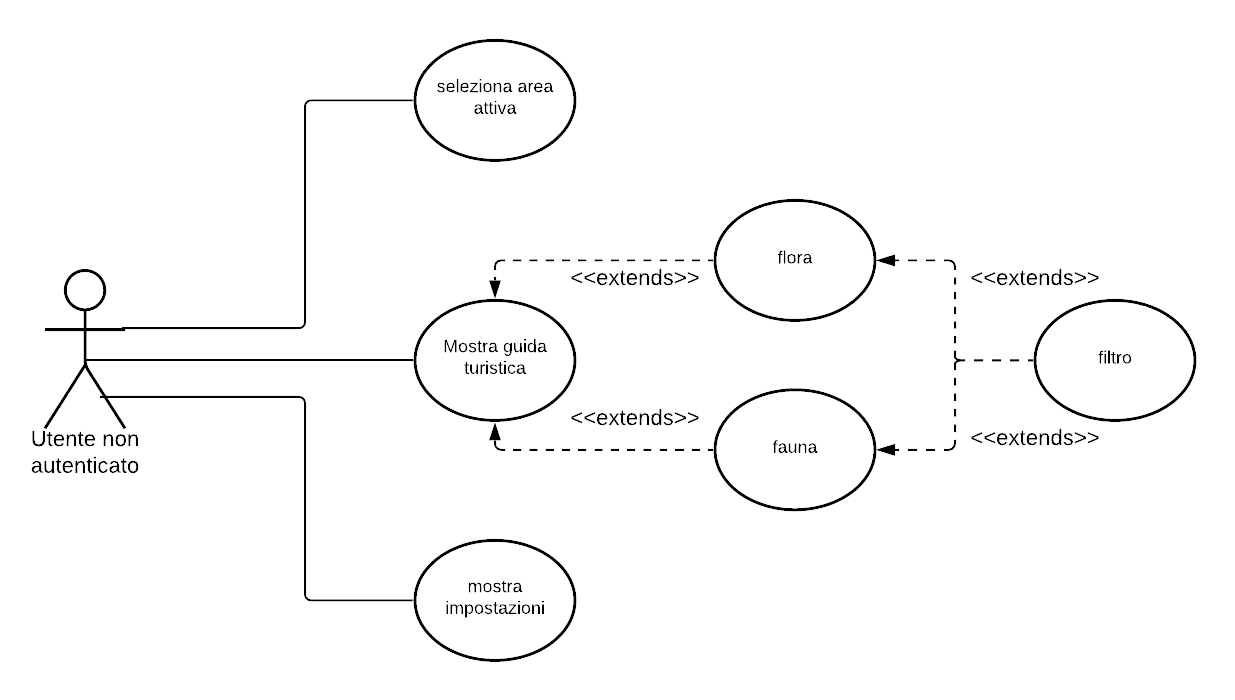
\includegraphics[scale=0.35]{Img/Utente_non_autenticato.png}
\end{figure}

\subsubsection*{Descrizione Use Case "seleziona area attiva"}
Questo use case descrive come l'utente può selezionare l'area in cui si trova.
\begin{enumerate}
    \item L'utente seleziona dal menù la voce "area attiva";
    \item Il sistema mostra la lista delle aree presenti nell'applicazione;
    \item L'utente seleziona l'area in cui si trova;
    \item Ora il sistema mostrerà le informazioni dell'area selezionata.
\end{enumerate}

\subsubsection*{Descrizione Use Case "mostra guida turistica"}
Questo use case descrive come vengono mostrate le informazioni di flora e fauna.
\begin{enumerate}
    \item L'utente seleziona dal menù la voce "flora" o "fauna";
    \item L'utente può applicare dei filtri: ordinamento (alfabetico, casuale), specie (protetta e non protetta) e popolazione (numero di esemplari: crescente o decrescente);
    \item Il sistema mostra tutte le specie presenti nell'ambiente;
    \item L'utente può selezionare una particolare specie per visualizzare una descrizione turistica.
\end{enumerate}

\subsubsection*{Descrizione Use Case "mostra impostazioni"}
Questo use case descrive cosa viene mostrato nelle impostazioni.
\begin{enumerate}
    \item L'utente seleziona dal menù la voce "impostazioni";
    \item Il sistema mostra una schermata dove l'utente può selezionare:
    \begin{itemize}
        \item disattiva notifiche;
        \item cambia lingua;
        \item assistenza;
        \item normative dati;
        \item informazioni app.
    \end{itemize}
\end{enumerate}

\subsubsection*{\underline{\large{Amministratore}}}

\begin{figure}[ht]
    \centering
    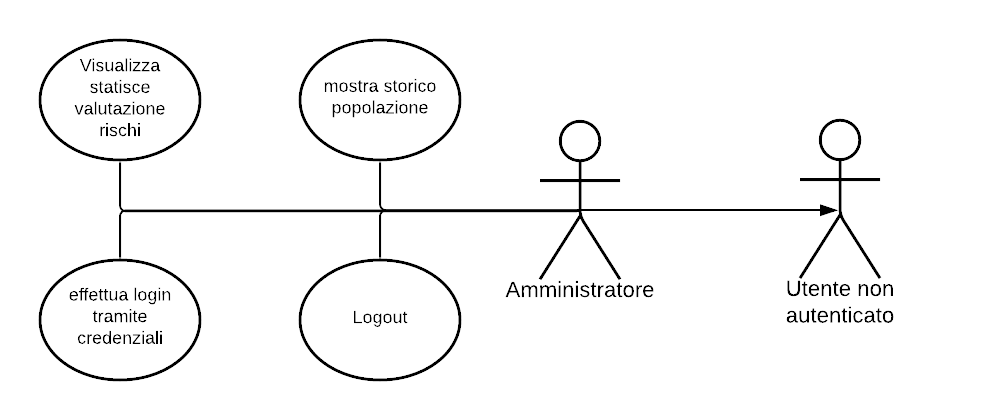
\includegraphics[scale=0.4]{Img/Amministratore.png}
\end{figure}

\subsubsection*{Descrizione Use Case "effettua login tramite credenziali"}
Questo use case descrive come avviene il login di un amministratore.
\begin{enumerate}
    \item L'amministratore fornisce agli sviluppatori un email valida;
    \item Gli sviluppatori creano un account per l'amministratore;
    \item L'amministratore dovrà effettuare il primo login utilizzando nome utente e OTP forniti via email;
    \item L'amministratore  seleziona dal menù la voce "login";
    \item L'amministratore deve inserire nome utente e password;
    \item Al primo login dovrà cambiare la password e successivamente ogni 30 giorni;
\end{enumerate}

\subsubsection*{Descrizione Use Case "visualizza statistiche valutazione rischi"}
Questo use case descrive come vengono mostrate le percentuali di rischio.
\begin{enumerate}
    \item L'amministratore seleziona dal menù "monitoraggio";
    \item Il sistema mostra a schermo le percentuali attuali dei vari rischi.
\end{enumerate}

\subsubsection*{Descrizione Use Case "mostra storico popolazione" \textbf{RF 2.5}}
Questo use case descrive come viene visualizzato lo storico della popolazione.
\begin{enumerate}
    \item L'amministratore seleziona dal menù "fauna";
    \item L'amministratore può applicare dei filtri: ordinamento (alfabetico, casuale), specie (protetta e non protetta) e popolazione (numero di esemplari: crescente o decrescente);
    \item Il sistema mostra tutte le specie presenti nell'ambiente;
    \item L'amministratore può selezionare una particolare specie per visualizzare le seguenti informazioni:
    \begin{itemize}
        \item istogramma popolazione/tempo (con scala del tempo selezionabile: anno, mese, giorno);
        \item mappa in cui è possibile visualizzare la posizione in tempo reale degli elementi specie selezionata presenti nell'area (se disponibile).
    \end{itemize}
\end{enumerate}

\subsubsection*{Descrizione Use Case "logout"}
Questo use case descrive come l'amministratore può effettuare il logout.
\begin{enumerate}
    \item L'amministratore ha a disposizione un pulsante nel menu chiamato "logout";
    \item L'amministratore può selezionare dal menù "area attiva";
    \item Se il sistema non identifica l'utente come amministratore nell'area selezionata viene effettuato il logout automatico.
\end{enumerate}

\phantomsection
\subsection*{RF 2.3 Monitoraggio e RF 2.4 Comunicazione}
\addcontentsline{toc}{subsection}{2.3 Monitoraggio e Comunicazione}
In questa sezione vengono descritte le azioni svolte dai seguenti attori:
\begin{itemize}
    \item Il sistema di calcolo probabilistico elabora i dati ricevuti dai sensori ambientali, come verrà spiegato successivamente;
    \item Il database memorizza i dati relativi alla flora, fauna, amministratori e i dati elaborati dal sistema di calcolo probabilistico;
    \item Il sistema di invio mail e di notifica si divide nei due casi espressi nelle pagine seguenti: disastri ambientali, fuga animali pericolosi.
\end{itemize}

\begin{figure}[ht]
    \centering
    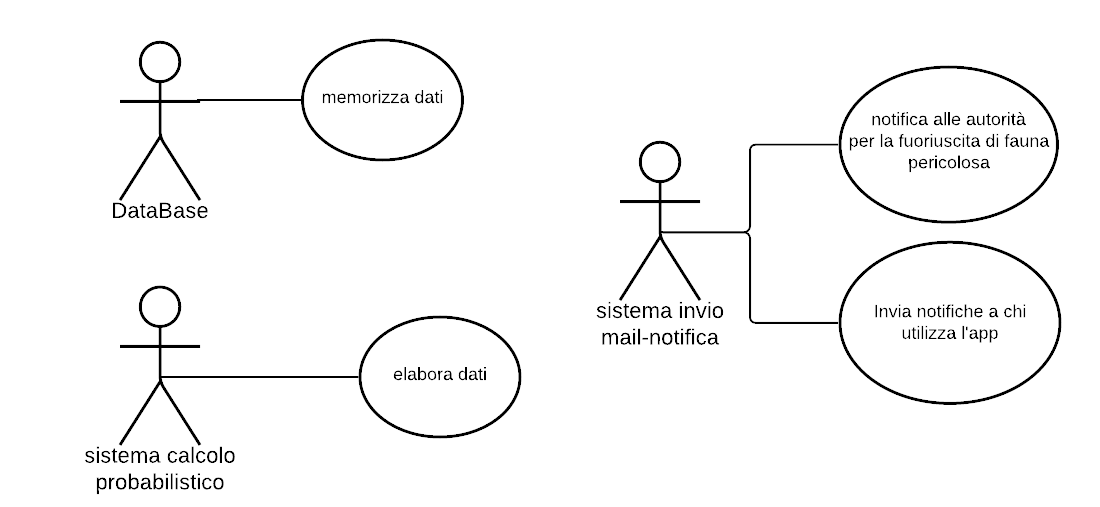
\includegraphics[scale=0.35]{Img/use_case_2_3_4.png}
\end{figure}

\pagebreak
\subsubsection*{Descrizione degli Use Case}

Il sistema di monitoraggio ambientale riceve dei dati elaborati sottoforma di percentuale dal sistema di calcolo probabilistico, elaborando i dati sulla probabilità dell'avverarsi dei seguenti rischi:
\begin{itemize}
    \item Allagamento
    \item Siccità
    \item Incendio 
    \item Svuotamento di risorse idriche
    \item Allarmi meteo
\end{itemize}
Nello schema sottostante viene descritta la \textbf{gestione dei rischi} da parte del sistema mediante Activity Diagram:

\begin{figure}[ht]
    \centering
    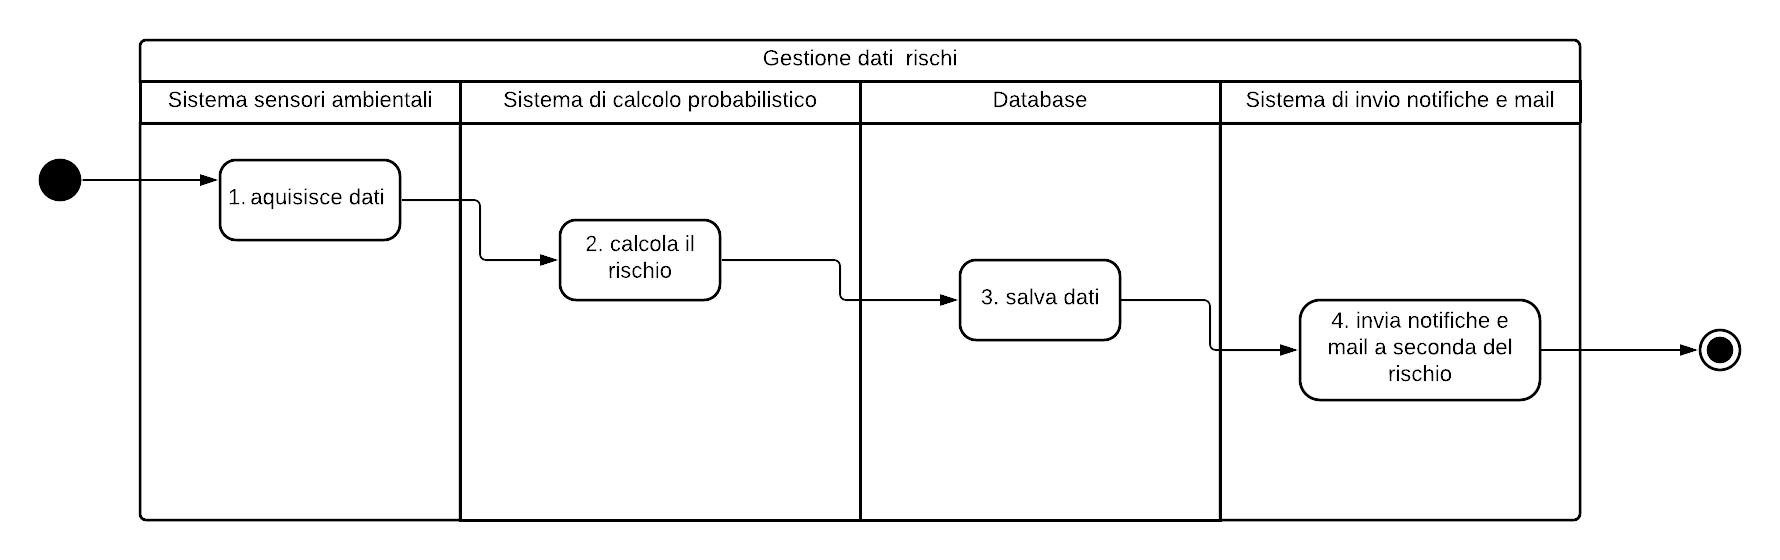
\includegraphics[scale=0.25]{Img/swim_gestione_rischi.png}
\end{figure}

La figura seguente, invece, descrive i vari casi a seconda delle analisi sul rischio ricevute. A ciascun livello sono associate determinate azioni.

\begin{figure}[ht]
    \centering
    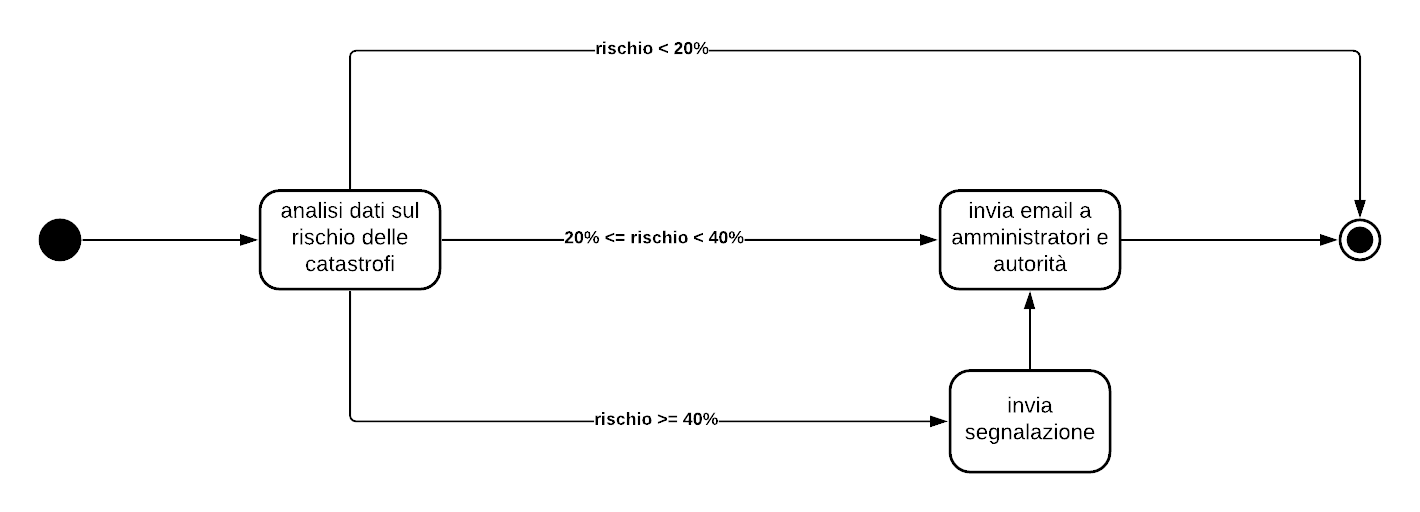
\includegraphics[scale=0.3]{Img/activity_rischi.png}
\end{figure}

\pagebreak

Il \textbf{sistema di sensori ambientali}, come precedentemente accennato, acquisisce dati e li fornisce al sistema di calcolo probabilistico. Il \textbf{sistema gps}, invece, indica la posizione e il numero di animali di medie e grandi dimensioni presenti nell'area, come spiegato nel diagramma seguente.

\begin{figure}[ht]
    \centering
    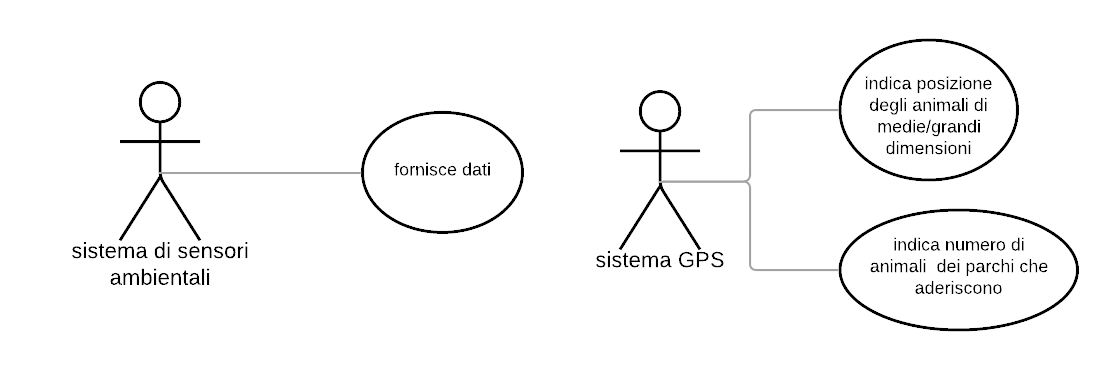
\includegraphics[scale=0.4]{Img/gestione_animali.png}
\end{figure}

\begin{figure}[ht]
    \centering
    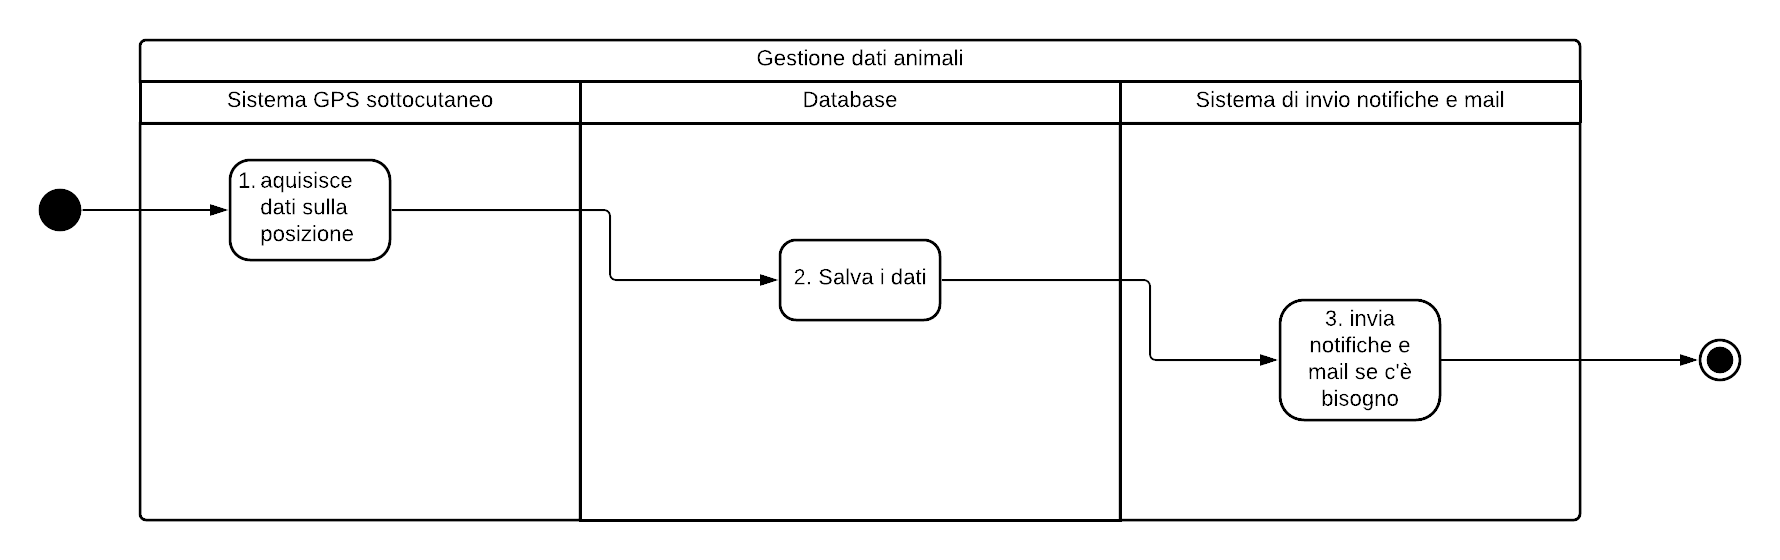
\includegraphics[scale=0.25]{Img/swim_gestione_animali.png}
\end{figure}

Il diagramma successivo analizza il caso in cui un animale fuoriesca dalla zona prestabilita.

\begin{figure}[ht]
    \centering
    
\includegraphics[scale=0.29]{Img/activity_animali.png}
\end{figure}
\section{Requisiti non funzionali}
Nella seguente sezione vengono riportati i requisiti non funzionali (RNF) del sistema.

\subsubsection*{RNF 3.1 Interfaccia}
\begin{table}[ht]
    \centering
    \begin{tabular}{| c | m{0.3\linewidth} | m{0.4\linewidth} |}
        \hline
        \rowcolor{Gray}
        \textbf{Proprietà} & \textbf{Descrizione} & \textbf{Misura} \\
        \hline
        Supporto multilingua & Tutte le schermate del software devono avere il supporto per tutte le lingue previste.  & Le schermate devono essere disponibili in: italiano, inglese, spagnolo, francese, tedesco, russo, cinese e giapponese. \\
        \hline
    \end{tabular}
\end{table}

\subsubsection*{RNF 3.2 Compatibilità}
\begin{table}[ht]
    \centering
    \begin{tabular}{| m{0.25\linewidth} | m{0.25\linewidth} | m{0.4\linewidth} |}
        \hline
        \rowcolor{Gray}
        \textbf{Proprietà} & \textbf{Descrizione} & \textbf{Misura} \\
        \hline
        Compatibilità con Web & Browser con i quali l'applicazione web deve essere compatibile & L'applicazione web deve essere compatibile con: browser: chrome (94.0.4606.61 e successivi), mozilla (91.0 e successivi), safari (15.0 e successivi) e microsoft edge (94.0.992.31 e successivi).\\
        \hline
        Compatibilità con iOS & Sistema operativo e versione a partire dalla quale l'applicazione web può essere utilizzata. & L'applicazione web deve essere compatibile con iOS 10 e successivi. \\
        \hline
        Compatibilità con Android & Sistema operativo e versione a partire dalla quale l'applicazione web può essere utilizzata. & L'applicazione web deve essere compatibile con Android 8.0 e successivi.\\
        \hline
    \end{tabular}
\end{table}

\subsubsection*{RNF 3.3 Efficienza}
\begin{table}[ht]
    \centering
    \begin{tabular}{| m{0.25\linewidth} | m{0.25\linewidth} | m{0.4\linewidth} |}
        \hline
        \rowcolor{Gray}
        \textbf{Proprietà} & \textbf{Descrizione} & \textbf{Misura} \\
        \hline
        Aggiornamento dati & Frequenza di aggiornamento dei dati riceviti dall'app. & I dati all'interno dell'applicazione devono essere aggiornati ogni 10 minuti .\\
        \hline
        Tempo di risposta geolocalizzazione & Tempo massimo di visualizzazione mappa animali  & Quando l'utente visualizza la mappa, deve essere aperta in meno di 4 secondi. \\
        \hline
       Transizione schermata & Tempo massimo di risposta per un interazione dell'utente con l'app. & La transizione tra una schermata e l'altra dovrà avvenire in meno di 2 secondi. \\
       \hline
    \end{tabular}
\end{table}

\pagebreak
\subsubsection*{RNF 3.4 Servizio}
\begin{table}[ht]
    \centering
    \begin{tabular}{| m{0.25\linewidth} | m{0.25\linewidth} | m{0.4\linewidth} |}
        \hline
        \rowcolor{Gray}
        \textbf{Proprietà} & \textbf{Descrizione} & \textbf{Misura} \\
        \hline
        Manutenzione & Tempo in cui l'applicazione non è accessibile per manutenzioni & Le manutenzioni devono essere eseguite entro 2 ore. \\
        \hline
    \end{tabular}
\end{table}

\subsubsection*{RNF 3.5 Sicurezza}
\begin{table}[ht]
    \centering
    \begin{tabular}{| m{0.25\linewidth} | m{0.25\linewidth} | m{0.4\linewidth} |}
        \hline
        \rowcolor{Gray}
        \textbf{Proprietà} & \textbf{Descrizione} & \textbf{Misura} \\
        \hline
        Cambio password & Tempo di validità della password & L'amministratore deve cambiare password ogni mese. \\
        \hline
    \end{tabular}
\end{table}

\end{document}
